\documentclass[12pt,a4paper]{article}

\usepackage[utf8]{inputenc}
\usepackage[T1]{fontenc}
\usepackage[brazilian]{babel}
\usepackage{amsmath,amssymb,amsfonts}
\usepackage{booktabs}
\usepackage{geometry}
\usepackage{hyperref}
\usepackage{longtable}
\usepackage{array}
\usepackage{xcolor}
\usepackage{enumitem}
\usepackage{graphicx}

\geometry{margin=2.5cm}
\setcounter{tocdepth}{3}
\setcounter{secnumdepth}{3}
\hypersetup{
  colorlinks=true,
  linkcolor=blue,
  citecolor=blue,
  urlcolor=blue
}

\newcommand{\R}{\mathbb{R}}
\newcommand{\E}{\mathbb{E}}
\newcommand{\Var}{\operatorname{Var}}
\newcommand{\Cov}{\operatorname{Cov}}
\newcommand{\tr}{\operatorname{tr}}
\newcommand{\argmin}{\operatorname*{arg\,min}}
\newcommand{\argmax}{\operatorname*{arg\,max}}
\newcommand{\one}{\mathbf{1}}
\newcommand{\what}{\widehat{w}}
\newcommand{\Sigmahat}{\widehat{\Sigma}}
\newcommand{\instituicao}{FGV EMAp}
\newcommand{\curso}{Ciência de Dados e Inteligência Artificial}
\newcommand{\autor}{Maria Eduarda Mesquita Magalhães}
\newcommand{\orientador}{Philip Thompson}
\newcommand{\titulo}{Robustificação de Carteiras de Mínima Variância com Ativos Brasileiros}
\newcommand{\subtitulo}{Uma aplicação da estimação robusta de $\Sigma w$ ao problema de Markowitz}

\begin{document}

\pagenumbering{gobble}

\begin{titlepage}
  \begin{center}
    \instituicao\\
    \curso

    \vfill

    {\large \autor}

    \vfill

    {\Large\bfseries \titulo\par}
    \vspace{0.5cm}
    {\large \subtitulo\par}

    \vfill

    \begin{flushright}
      \begin{minipage}{0.52\textwidth}
        Trabalho em formato de relatório técnico-científico apresentado como material de
        apoio para estudo de Estatística Robusta aplicada à otimização de carteiras.

        \vspace{0.4cm}
        Orientador(a): \orientador
      \end{minipage}
    \end{flushright}

    \vfill

    Brasil\\
    \today
  \end{center}
\end{titlepage}

\pagenumbering{roman}

\section*{Resumo}
\addcontentsline{toc}{section}{Resumo}
Este trabalho investiga se carteiras global minimum variance (GMV) robustificadas por
estimação robusta da ação da covariância, $\Sigma w$, apresentam menor instabilidade de pesos
e melhor desempenho líquido fora da amostra do que carteiras GMV baseadas em covariância
amostral e estimadores de shrinkage, quando aplicadas a ativos do mercado brasileiro. O estudo
reproduz a lógica central do artigo \emph{Robustifying Markowitz}, adaptando o universo
empírico para ativos brasileiros, usando janelas móveis de $T=252$ e $T=500$ dias,
rebalanceamento mensal, custos de transação de 50 pontos-base e comparação com benchmarks
como Equal Weight, GMV amostral, GMV Long Only, shrinkage linear, nonlinear shrinkage e índice
de mercado. Além de documentar a metodologia computacional adotada, o texto apresenta as
equações fundamentais de Markowitz, projected gradient descent, projeção
orçamentária, estimadores robustos sob caudas pesadas e agregação Hopkins--Li--Zhang (HLZ). Os
resultados indicam que a carteira robusta melhora a estabilidade frente à GMV amostral e aos
métodos de shrinkage em termos de turnover, apresentando desempenho líquido competitivo e, em
alguns cenários, superior em Sharpe ou Calmar.

\vspace{0.3cm}
\noindent\textbf{Palavras-chave:} Estatística Robusta; Markowitz; GMV; caudas pesadas;
shrinkage; mercado brasileiro.

\newpage

\section*{Abstract}
\addcontentsline{toc}{section}{Abstract}
This report studies whether robustified global minimum variance portfolios, based on robust
estimation of the covariance action $\Sigma w$, display lower weight instability and better
net out-of-sample performance than GMV portfolios based on sample covariance and shrinkage
estimators when applied to Brazilian equities. The project follows the central logic of
\emph{Robustifying Markowitz}, replacing the original empirical universe with Brazilian
assets, using rolling windows of $T=252$ and $T=500$ trading days, monthly rebalancing,
transaction costs of 50 basis points and comparisons against standard benchmarks. The report
also explains the mathematical structure of the repository, including GMV optimization,
projected gradient descent, budget projection, robust estimation under heavy tails and the
Hopkins--Li--Zhang spectral reweighting procedure. The empirical results suggest that the
robust GMV portfolio reduces turnover relative to sample GMV and shrinkage methods while
remaining competitive, and sometimes superior, in risk-adjusted net performance.

\vspace{0.3cm}
\noindent\textbf{Keywords:} Robust Statistics; Markowitz; GMV; heavy tails; shrinkage;
Brazilian stock market.

\newpage
\tableofcontents
\newpage
\listoffigures
\newpage
\listoftables
\newpage
\pagenumbering{arabic}

\section{Visão geral do projeto}

O projeto parte de uma pergunta prática:

\begin{quote}
Como construir carteiras de mínima variância que sejam menos sensíveis a erros de estimação,
caudas pesadas e mudanças bruscas nos pesos, usando dados do mercado brasileiro?
\end{quote}

O artigo \emph{Robustifying Markowitz} argumenta que a implementação clássica de Markowitz,
baseada em média e covariância amostrais, pode gerar pesos instáveis e altos custos de
transação. A contribuição principal do artigo não é simplesmente trocar a covariância amostral
por uma ``covariância robusta''. A ideia central é mais sutil:

\begin{center}
\fbox{\parbox{0.88\textwidth}{
Em vez de estimar uma matriz de covariância robusta completa e depois invertê-la, estima-se
robustamente apenas a ação da covariância sobre o vetor de pesos atual, isto é, $\Sigma w$,
dentro de um algoritmo iterativo de gradiente projetado.
}}
\end{center}

Neste trabalho, essa lógica foi aplicada a um universo brasileiro congelado baseado no
Ibovespa. O experimento roda duas janelas de estimação, $T=252$ e $T=500$, usa custo de
transação de 50 bps e compara a carteira robusta contra benchmarks usuais.

\subsection{Pergunta de pesquisa}

A pergunta que orienta este trabalho é:

\begin{quote}
Carteiras GMV robustificadas por estimação robusta de $\Sigma w$ apresentam menor
instabilidade de pesos e melhor desempenho líquido fora da amostra do que carteiras GMV
baseadas em covariância amostral e shrinkage, quando aplicadas a ativos do mercado brasileiro?
\end{quote}

Essa pergunta é adequada porque conecta diretamente a teoria estatística à aplicação empírica.
O objeto $\Sigma w$ é o gradiente do problema GMV; portanto, estimá-lo bem é essencial para
obter pesos estáveis. Ao mesmo tempo, o desempenho fora da amostra e o turnover verificam se a
melhora matemática se traduz em uma carteira operacionalmente útil.

\subsection{Hipótese de pesquisa}

A hipótese de pesquisa adotada é:

\begin{quote}
\textbf{Hipótese de pesquisa:} carteiras GMV robustificadas por estimação robusta de
$\Sigma w$ apresentam menor instabilidade de pesos e melhor desempenho líquido fora da amostra
do que carteiras GMV baseadas em covariância amostral e shrinkage, quando aplicadas a ativos
do mercado brasileiro.
\end{quote}

Em termos empíricos, essa hipótese será avaliada por métricas de desempenho líquido, como
Sharpe e Calmar, e por métricas de estabilidade, como turnover, target turnover e distribuição
dos pesos.

\subsection{Objetivos}

O objetivo geral é adaptar a lógica do artigo \emph{Robustifying Markowitz} para um universo de
ativos brasileiros e avaliar se a robustificação melhora a estabilidade e o desempenho líquido
das carteiras GMV.

Os objetivos específicos são:

\begin{enumerate}[leftmargin=*]
  \item preparar uma base de preços ajustados de ativos brasileiros e do índice de mercado;
  \item calcular retornos e construir janelas móveis de estimação;
  \item implementar carteiras EW, GMV amostral, GMV Long Only, GMV com shrinkage linear, GMV
  com nonlinear shrinkage e GMV Robust;
  \item implementar a otimização por projected gradient descent com projeção orçamentária;
  \item aplicar estimação robusta de $\Sigma w$ usando blocos, truncagem e agregação HLZ;
  \item executar backtests com rebalanceamento mensal e custos de transação;
  \item comparar as carteiras por retorno, volatilidade, Sharpe, Calmar, drawdown, turnover e
  estatísticas dos pesos.
\end{enumerate}

\subsection{Contribuição do trabalho}

A contribuição deste trabalho é dupla. Do ponto de vista didático, o relatório traduz a
matemática do artigo para uma sequência implementável e comentada. Do ponto de vista empírico,
o projeto aplica a metodologia a ativos brasileiros, mantendo a estrutura central do paper:
não se estima uma covariância robusta completa para depois invertê-la; estima-se robustamente a
ação $\Sigma w$ dentro do algoritmo de otimização.

\subsection{Procedimento metodológico}

O experimento foi conduzido de forma sequencial, da preparação dos dados à análise dos
resultados. A Tabela~\ref{tab:procedimento-metodologico} resume a ordem das etapas.

\begin{longtable}{p{0.12\textwidth}p{0.78\textwidth}}
\caption{Procedimento metodológico executado no estudo.}
\label{tab:procedimento-metodologico}\\
\toprule
\textbf{Etapa} & \textbf{Descrição} \\
\midrule
1 & Seleção do universo brasileiro de ações, com congelamento dos ativos elegíveis para manter a reprodutibilidade. \\
2 & Coleta e limpeza dos preços ajustados, removendo séries insuficientes ou incompatíveis com as janelas de estimação. \\
3 & Cálculo dos retornos simples diários a partir dos preços ajustados. \\
4 & Construção de janelas móveis de estimação com $T=252$ e $T=500$ observações. \\
5 & Estimação das matrizes ou ações de covariância necessárias para cada carteira: covariância amostral, shrinkage linear, nonlinear shrinkage e estimação robusta de $\Sigma w$. \\
6 & Otimização das carteiras EW, GMV amostral, GMV Long Only, GMV Linear Shrinkage, GMV Nonlinear Shrinkage e GMV Robust. \\
7 & Rebalanceamento mensal das carteiras, mantendo os pesos entre datas de rebalanceamento. \\
8 & Cálculo dos retornos brutos e líquidos, descontando custo de transação de 50 pontos-base proporcional ao turnover. \\
9 & Cálculo das métricas de desempenho, risco e estabilidade dos pesos. \\
10 & Geração das tabelas, figuras e interpretação dos resultados em relação à hipótese de pesquisa. \\
\bottomrule
\end{longtable}

\section{Por que Estatística Robusta entra no problema?}

\subsection{O problema das caudas pesadas}

Em muitos modelos elementares, assume-se que retornos financeiros são aproximadamente
normais. Na prática, retornos de ativos frequentemente têm:

\begin{itemize}[leftmargin=*]
  \item assimetria;
  \item curtose elevada;
  \item outliers;
  \item períodos de estresse em que correlações mudam rapidamente.
\end{itemize}

Dizemos que uma distribuição possui \emph{caudas pesadas} quando eventos extremos são mais
prováveis do que seriam em uma distribuição normal. Isso afeta diretamente estimadores
clássicos como a média amostral e a covariância amostral.

Se $X_1,\dots,X_T \in \R^N$ são vetores de retornos, a covariância amostral é
\begin{equation}
  \Sigmahat
  =
  \frac{1}{T-1}\sum_{t=1}^{T}(X_t-\bar X)(X_t-\bar X)^\top,
  \qquad
  \bar X = \frac{1}{T}\sum_{t=1}^{T} X_t.
\end{equation}

Sob normalidade e amostras grandes, esse estimador é natural. Sob caudas pesadas, poucos
observações extremas podem deslocar muito $\Sigmahat$. Em Markowitz, pequenas perturbações
em $\Sigmahat$ podem gerar grandes mudanças em $w$, pois a solução clássica envolve uma
inversão de matriz.

\subsection{Robustez}

Um estimador robusto é desenhado para manter desempenho razoável quando as hipóteses
ideais falham. Neste projeto, robustez significa principalmente:

\begin{itemize}[leftmargin=*]
  \item reduzir a influência de observações extremas;
  \item evitar a inversão direta de matrizes mal condicionadas;
  \item estabilizar pesos ao longo do tempo;
  \item reduzir turnover e custos de transação.
\end{itemize}

Essa visão vem da literatura moderna de estimação robusta em alta dimensão, incluindo
Lugosi e Mendelson, Hopkins, Li e Zhang, e os resultados usados pelo artigo
\emph{Robustifying Markowitz}.

\section{Carteira de mínima variância global}

\subsection{Retornos e pesos}

Considere $N$ ativos. Em um dia $t$, escrevemos o vetor de retornos como
\begin{equation}
  X_t = (r_{1,t}, r_{2,t}, \dots, r_{N,t})^\top \in \R^N.
\end{equation}

Uma carteira é um vetor de pesos
\begin{equation}
  w = (w_1,\dots,w_N)^\top,
\end{equation}
em que $w_i$ é a fração alocada no ativo $i$. A restrição orçamentária é
\begin{equation}
  \one^\top w = 1.
\end{equation}

O retorno da carteira no dia $t$ é
\begin{equation}
  R_{p,t} = w^\top X_t.
\end{equation}

Se $\Sigma = \Cov(X_t)$ é a matriz de covariância populacional, a variância da carteira é
\begin{equation}
  \Var(R_{p,t}) = w^\top \Sigma w.
\end{equation}

\subsection{Problema GMV}

A carteira global minimum variance (GMV) minimiza risco sem usar estimativas de retorno
esperado:
\begin{equation}
  w^\star
  =
  \argmin_{w \in \R^N}
  \frac{1}{2} w^\top \Sigma w
  \quad \text{sujeito a} \quad
  \one^\top w = 1.
  \label{eq:gmv}
\end{equation}

O fator $1/2$ é usado por conveniência, pois o gradiente fica
\begin{equation}
  \nabla_w \left(\frac{1}{2}w^\top\Sigma w\right)
  =
  \Sigma w.
\end{equation}

Quando $\Sigma$ é inversível, a solução fechada é
\begin{equation}
  w^\star =
  \frac{\Sigma^{-1}\one}{\one^\top \Sigma^{-1}\one}.
  \label{eq:gmv_closed}
\end{equation}

Na prática, $\Sigma$ é desconhecida e substituída por algum estimador. O problema é que
\eqref{eq:gmv_closed} pode ser instável quando a covariância estimada é ruidosa ou mal
condicionada.

\section{Projected Gradient Descent}

O artigo usa projected gradient descent (PGD) para resolver o problema GMV sem depender
diretamente de uma inversão matricial. A atualização ideal, se $\Sigma$ fosse conhecida, seria
\begin{equation}
  w_s
  =
  \Pi_1\left[
    w_{s-1} - \eta \Sigma w_{s-1}
  \right],
  \qquad s=1,2,\dots,
  \label{eq:pgd}
\end{equation}
em que $\eta>0$ é o passo e $\Pi_1$ é a projeção no hiperplano $\one^\top w = 1$.

\subsection{Projeção orçamentária}

A projeção usada no artigo é
\begin{equation}
  \Pi_1 x
  =
  \left(I - \frac{1}{N}\one\one^\top\right)x
  +
  \frac{1}{N}\one.
  \label{eq:proj_budget}
\end{equation}

Essa projeção garante que os pesos somem 1, mas \textbf{não} impõe $w_i \ge 0$. Portanto,
ela permite posições vendidas. Isso é importante: a carteira robusta do artigo procura
estabilidade sem impor uma restrição long-only a priori.

\section{\texorpdfstring{A ideia robusta: estimar $\Sigma w$, não $\Sigma$}{A ideia robusta: estimar Sigma w, nao Sigma}}

O ponto mais importante do artigo é trocar a estimação de uma matriz inteira por uma
estimação robusta da ação dessa matriz:
\begin{equation}
  \Sigma w.
\end{equation}

Se $\E X = 0$, então
\begin{equation}
  \Sigma w
  =
  \E\left[XX^\top w\right]
  =
  \E\left[X(X^\top w)\right].
  \label{eq:sigma_action}
\end{equation}

Assim, para um $w$ fixo, estimar $\Sigma w$ vira um problema de estimação robusta de média
vetorial aplicada aos vetores
\begin{equation}
  Y_t(w) = X_t(X_t^\top w).
\end{equation}

No PGD robusto, a atualização torna-se
\begin{equation}
  w_s
  =
  \Pi_1\left[
    w_{s-1} - \eta \widehat a(w_{s-1})
  \right],
  \label{eq:robust_pgd}
\end{equation}
em que $\widehat a(w)$ é um estimador robusto de $\Sigma w$.

\section{\texorpdfstring{Como o projeto estima $\Sigma w$}{Como o projeto estima Sigma w}}

O artigo descreve quatro ideias principais:

\begin{enumerate}[leftmargin=*]
  \item centralizar as observações sem estimar a média;
  \item dividir a amostra em blocos;
  \item truncar observações extremas por norma;
  \item agregar os vetores de bloco via spectral sample reweighting do tipo HLZ.
\end{enumerate}

\subsection{Centralização por pares}

Para evitar depender de uma estimativa da média, o artigo usa diferenças pareadas:
\begin{equation}
  \widetilde X_1 = \frac{X_1-X_2}{\sqrt{2}},
  \quad
  \widetilde X_2 = \frac{X_3-X_4}{\sqrt{2}},
  \quad \dots
\end{equation}

Se $X_i$ são independentes com covariância $\Sigma$, então
\begin{equation}
  \Cov\left(\frac{X_1-X_2}{\sqrt{2}}\right)
  =
  \frac{1}{2}\left(\Cov(X_1)+\Cov(X_2)\right)
  =
  \Sigma.
\end{equation}

Logo, a transformação remove a média, mas preserva a covariância. Essa é a primeira etapa da
estimação robusta usada no experimento.

\subsection{Blocos e truncagem}

Depois da centralização, os dados são divididos em $\ell$ blocos. O artigo usa
heuristicamente $\ell=10$ e $\epsilon=1/3$ nos experimentos empíricos. O projeto segue essa
escolha.

Para cada bloco $B_j$, calcula-se uma ação de covariância robustificada:
\begin{equation}
  \widehat\Sigma_j w
  =
  \frac{1}{|B_j|}
  \sum_{i\in B_j}
  \widetilde X_i(\widetilde X_i^\top w)
  \mathbf{1}_{\|\widetilde X_i\|\le D}.
  \label{eq:block_action}
\end{equation}

No projeto, o limiar $D$ é operacionalizado por quantil da norma, via \texttt{trim\_quantile}.
Isso é uma escolha prática: o artigo observa que o parâmetro teórico exato depende de
quantidades desconhecidas, como posto efetivo e constantes de cauda.

\subsection{Agregação HLZ / spectral sample reweighting}

O projeto implementa um agregador baseado em Hopkins, Li e Zhang (HLZ), especificamente
na formulação de \emph{spectral sample reweighting}. A entrada do agregador são os vetores
de bloco:
\begin{equation}
  Z_j = \widehat\Sigma_j w,
  \qquad j=1,\dots,\ell.
\end{equation}

A ideia é encontrar pesos $u_j$ e um centro $\nu$ que minimizem a maior direção de
dispersão:
\begin{equation}
  \lambda_{\max}
  \left(
    \sum_{j=1}^{\ell}
    u_j (Z_j-\nu)(Z_j-\nu)^\top
  \right).
  \label{eq:spectral_center}
\end{equation}

Os pesos pertencem ao simplex capado
\begin{equation}
  W_{\ell,\epsilon}
  =
  \left\{
    u\in\Delta_\ell:
    \|u\|_\infty \le \frac{1}{(1-\epsilon)\ell}
  \right\}.
  \label{eq:capped_simplex}
\end{equation}

Essa restrição impede que o algoritmo coloque peso demais em poucos blocos.

\subsubsection{Passos do algoritmo HLZ usado no experimento}

A versão operacional do algoritmo tipo Filter/MWU segue os seguintes passos:

\begin{enumerate}[leftmargin=*]
  \item Comece com pesos uniformes $u_j^{(0)}=1/\ell$.
  \item Calcule o centro ponderado
  \begin{equation}
    \nu^{(t)} = \sum_{j=1}^{\ell} u_j^{(t)} Z_j.
  \end{equation}
  \item Calcule a matriz de dispersão ponderada
  \begin{equation}
    M^{(t)}
    =
    \sum_{j=1}^{\ell}
    u_j^{(t)}
    (Z_j-\nu^{(t)})(Z_j-\nu^{(t)})^\top.
  \end{equation}
  \item Encontre o autovetor $v^{(t)}$ associado ao maior autovalor de $M^{(t)}$.
  \item Defina perdas quadráticas
  \begin{equation}
    \tau_j^{(t)}
    =
    \left(v^{(t)\top}(Z_j-\nu^{(t)})\right)^2.
  \end{equation}
  \item Atualize pesos por multiplicative weights:
  \begin{equation}
    \tilde u_j^{(t+1)}
    =
    u_j^{(t)}
    \left(
      1-\eta\frac{\tau_j^{(t)}}{\rho}
    \right).
  \end{equation}
  \item Projete por divergência KL no conjunto $W_{\ell,\epsilon}$:
  \begin{equation}
    u^{(t+1)}
    =
    \argmin_{u\in W_{\ell,\epsilon}}
    \mathrm{KL}(u\,\|\,\tilde u^{(t+1)}).
  \end{equation}
  \item Retorne a iteração com menor $\lambda_{\max}(M^{(t)})$.
\end{enumerate}

\section{Benchmarks implementados}

O projeto compara a carteira robusta com os benchmarks do artigo.

\subsection{Equal Weight}

A carteira equally weighted (EW) aloca igualmente:
\begin{equation}
  w_i = \frac{1}{N}, \qquad i=1,\dots,N.
\end{equation}

Ela é simples, robusta a erro de estimação e frequentemente difícil de superar em estudos
empíricos.

\subsection{GMV amostral}

Usa a covariância amostral:
\begin{equation}
  \Sigmahat
  =
  \frac{1}{T-1}
  \sum_{t=1}^{T}
  (X_t-\bar X)(X_t-\bar X)^\top.
\end{equation}

Os pesos são:
\begin{equation}
  \what_{\mathrm{GMV}}
  =
  \frac{\Sigmahat^{-1}\one}{\one^\top\Sigmahat^{-1}\one}.
\end{equation}

\subsection{GMV Long Only}

Resolve o mesmo problema de mínima variância, mas com restrição adicional:
\begin{equation}
  w_i \ge 0,
  \qquad
  \one^\top w=1.
\end{equation}

Neste estudo, essa carteira é resolvida por projected gradient descent no simplex.

\subsection{Linear Shrinkage}

O estimador de Ledoit e Wolf combina a covariância amostral com um alvo estruturado:
\begin{equation}
  \Sigmahat_{\mathrm{lin}}
  =
  \rho F + (1-\rho)\Sigmahat.
\end{equation}

Na implementação empírica, usa-se o estimador linear de Ledoit--Wolf com alvo estruturado.

\subsection{Nonlinear Shrinkage}

O nonlinear shrinkage preserva os autovetores amostrais e transforma os autovalores de modo
não linear. Se
\begin{equation}
  \Sigmahat = U \Lambda U^\top,
\end{equation}
então o estimador tem a forma
\begin{equation}
  \Sigmahat_{\mathrm{nlin}}
  =
  U \widetilde\Lambda U^\top,
\end{equation}
em que os autovalores em $\widetilde\Lambda$ são versões encolhidas de forma não linear.

O estudo usa uma versão espectral inspirada em Ledoit e Wolf (2017), baseada em uma
aproximação suavizada do Stieltjes transform. A matriz resultante foi verificada quanto à
simetria e positividade dos autovalores, propriedades necessárias para que o estimador seja
compatível com um problema de variância.

\subsection{GMV Robust}

A carteira robusta é:
\begin{equation}
  w_0 = \frac{1}{N}\one,
  \qquad
  w_s
  =
  \Pi_1
  \left[
    w_{s-1}
    -
    \eta \widehat a(w_{s-1})
  \right],
\end{equation}
em que $\widehat a(w)$ é o estimador robusto de $\Sigma w$ construído por blocos e HLZ.

\section{Dados brasileiros}

O universo brasileiro usado no experimento foi congelado após a aplicação dos filtros de
histórico. Ao final desse procedimento, permaneceram 54 ativos elegíveis. Congelar o universo
é importante porque a carteira teórica do Ibovespa muda ao longo do tempo. Sem congelamento,
uma repetição futura do estudo poderia usar outro conjunto de ativos e produzir resultados
não comparáveis.

O benchmark de mercado é o Ibovespa, usado como referência para avaliar se as carteiras
otimizadas entregam desempenho competitivo contra uma alternativa ampla e observável do
mercado brasileiro.
\begin{equation}
  I_t = \text{nível do Ibovespa no dia } t.
\end{equation}

\section{Backtest}

\subsection{Janelas móveis}

O artigo usa janelas de 12 e 24 meses, aproximadamente:
\begin{equation}
  T=252
  \quad \text{e} \quad
  T=500.
\end{equation}

As duas janelas foram avaliadas separadamente. Para cada data de rebalanceamento, usa-se
apenas a informação disponível nos $T$ dias anteriores, estima-se a carteira e aplica-se essa
alocação ao período seguinte. Esse desenho evita usar informação futura no cálculo dos pesos.

\subsection{Retornos brutos e líquidos}

O retorno bruto da carteira no dia $t$ é
\begin{equation}
  R_{p,t}^{\mathrm{gross}} = w^\top X_t.
\end{equation}

O retorno líquido desconta custos de transação no dia de rebalanceamento:
\begin{equation}
  R_{p,t}^{\mathrm{net}}
  =
  R_{p,t}^{\mathrm{gross}}
  -
  c \cdot \mathrm{TO}_t,
\end{equation}
em que $c=0.005$ corresponde a 50 bps, como no artigo.

\subsection{Turnover}

O turnover mede quanto a carteira precisa negociar para sair dos pesos imediatamente antes
do rebalanceamento e chegar aos novos pesos-alvo.

Se $w_{j,l+}$ é o peso do ativo $j$ imediatamente antes do rebalanceamento e $w_{j,l+1}$ é
o novo peso-alvo, então:
\begin{equation}
  \mathrm{TO}
  =
  \frac{1}{L}
  \sum_{l=1}^{L}
  \sum_{j=1}^{N}
  |w_{j,l+1} - w_{j,l+}|.
\end{equation}

O target turnover remove o efeito do drift de preços:
\begin{equation}
  \mathrm{TTO}
  =
  \frac{1}{L}
  \sum_{l=1}^{L}
  \sum_{j=1}^{N}
  |w_{j,l+1} - w_{j,l}|.
\end{equation}

\section{Métricas}

\subsection{Riqueza acumulada}

Com riqueza inicial $W_0=1$, a riqueza acumulada é
\begin{equation}
  W_t = \prod_{s=1}^{t}(1+R_{p,s}).
\end{equation}

\subsection{Volatilidade anualizada}

Se os retornos são diários:
\begin{equation}
  \sigma_{\mathrm{ann}}
  =
  \sqrt{252}\,\mathrm{sd}(R_{p,t}).
\end{equation}

\subsection{Sharpe Ratio}

Com taxa livre de risco diária igual a zero no projeto:
\begin{equation}
  \mathrm{SR}
  =
  \sqrt{252}
  \frac{\bar R_p}{\mathrm{sd}(R_p)}.
\end{equation}

\subsection{Maximum Drawdown e Calmar}

O drawdown em $t$ é
\begin{equation}
  \mathrm{DD}_t
  =
  \frac{W_t}{\max_{s\le t}W_s}-1.
\end{equation}

O máximo drawdown é o menor valor dessa série. O Calmar ratio é
\begin{equation}
  \mathrm{Calmar}
  =
  \frac{\text{retorno anualizado}}{|\mathrm{MDD}|}.
\end{equation}

\subsection{Estatísticas dos pesos}

O projeto calcula:
\begin{itemize}[leftmargin=*]
  \item peso mínimo médio;
  \item peso máximo médio;
  \item desvio padrão médio dos pesos;
  \item distância média para EW, chamada \texttt{mad\_ew};
  \item amplitude média \texttt{max\_minus\_min};
  \item número efetivo de ativos.
\end{itemize}

O número efetivo de ativos é
\begin{equation}
  N_{\mathrm{eff}}
  =
  \frac{1}{\sum_{i=1}^{N}w_i^2}.
\end{equation}

\section{Testes estatísticos}

O artigo reporta p-valores em relação à carteira GMV Robust. O projeto implementa:

\begin{itemize}[leftmargin=*]
  \item t-test pareado para turnover e target turnover;
  \item teste HAC/Newey--West via delta method para Sharpe;
  \item teste HAC/Newey--West via delta method para variância.
\end{itemize}

Para Sharpe e variância, usa-se a série de momentos:
\begin{equation}
  m_t = (R_{x,t}, R_{y,t}, R_{x,t}^2, R_{y,t}^2),
\end{equation}
em que $x$ é a carteira comparada e $y$ é a GMV Robust. A covariância de longo prazo dos
momentos é estimada por Newey--West:
\begin{equation}
  \widehat\Omega
  =
  \widehat\Gamma_0
  +
  \sum_{\ell=1}^{q}
  \left(1-\frac{\ell}{q+1}\right)
  \left(
    \widehat\Gamma_\ell
    +
    \widehat\Gamma_\ell^\top
  \right).
\end{equation}

O delta method transforma a incerteza dos momentos em incerteza da estatística desejada.

\section{Resultados empíricos recentes}

As tabelas abaixo resumem resultados líquidos obtidos no projeto com dados brasileiros,
universo congelado e custo de transação de 50 bps.

\subsection{\texorpdfstring{Janela $T=252$}{Janela T=252}}

\begin{table}[htbp]
\centering
\caption{Resultados líquidos das carteiras para janela de estimação $T=252$.}
\label{tab:resultados-252}
\begin{tabular}{lrrrr}
\toprule
Carteira & Sharpe & Calmar & TO & TTO \\
\midrule
EW & 0.509 & 0.210 & 0.065 & 0.000 \\
GMV & 0.412 & 0.186 & 0.988 & 0.956 \\
GMV Long Only & 0.537 & 0.218 & 0.076 & 0.042 \\
GMV Linear Shrinkage & 0.654 & 0.334 & 0.528 & 0.503 \\
GMV Nonlinear Shrinkage & 0.553 & 0.263 & 0.733 & 0.705 \\
GMV Robust & 0.713 & 0.317 & 0.370 & 0.358 \\
Index & 0.468 & 0.182 & 0.000 & 0.000 \\
\bottomrule
\end{tabular}
\end{table}

Para $T=252$, a carteira robusta apresenta Sharpe superior aos benchmarks listados e turnover
menor que GMV e shrinkage, mas maior que EW e GMV Long Only. O resultado é coerente com a
ideia do artigo: a robustificação reduz instabilidade em relação aos métodos plug-in e
shrinkage, sem impor a restrição long-only.

\subsubsection{Gráficos para \texorpdfstring{$T=252$}{T=252}}

A Figura~\ref{fig:wealth252} mostra a riqueza acumulada líquida das carteiras. Essa figura
é a tradução visual da sequência
\[
  V_t = \prod_{s=1}^{t}(1+r^{\mathrm{net}}_s),
\]
em que $r^{\mathrm{net}}_s$ já desconta o custo de transação. Para alunos iniciantes, é útil
ler esse gráfico como uma simulação de ``um real investido'' no início do backtest. Curvas
mais altas indicam maior crescimento acumulado, mas a inclinação e as quedas também importam:
uma curva que cresce muito e depois cai fortemente pode ter Sharpe ou Calmar pior.

\begin{figure}[htbp]
  \centering
  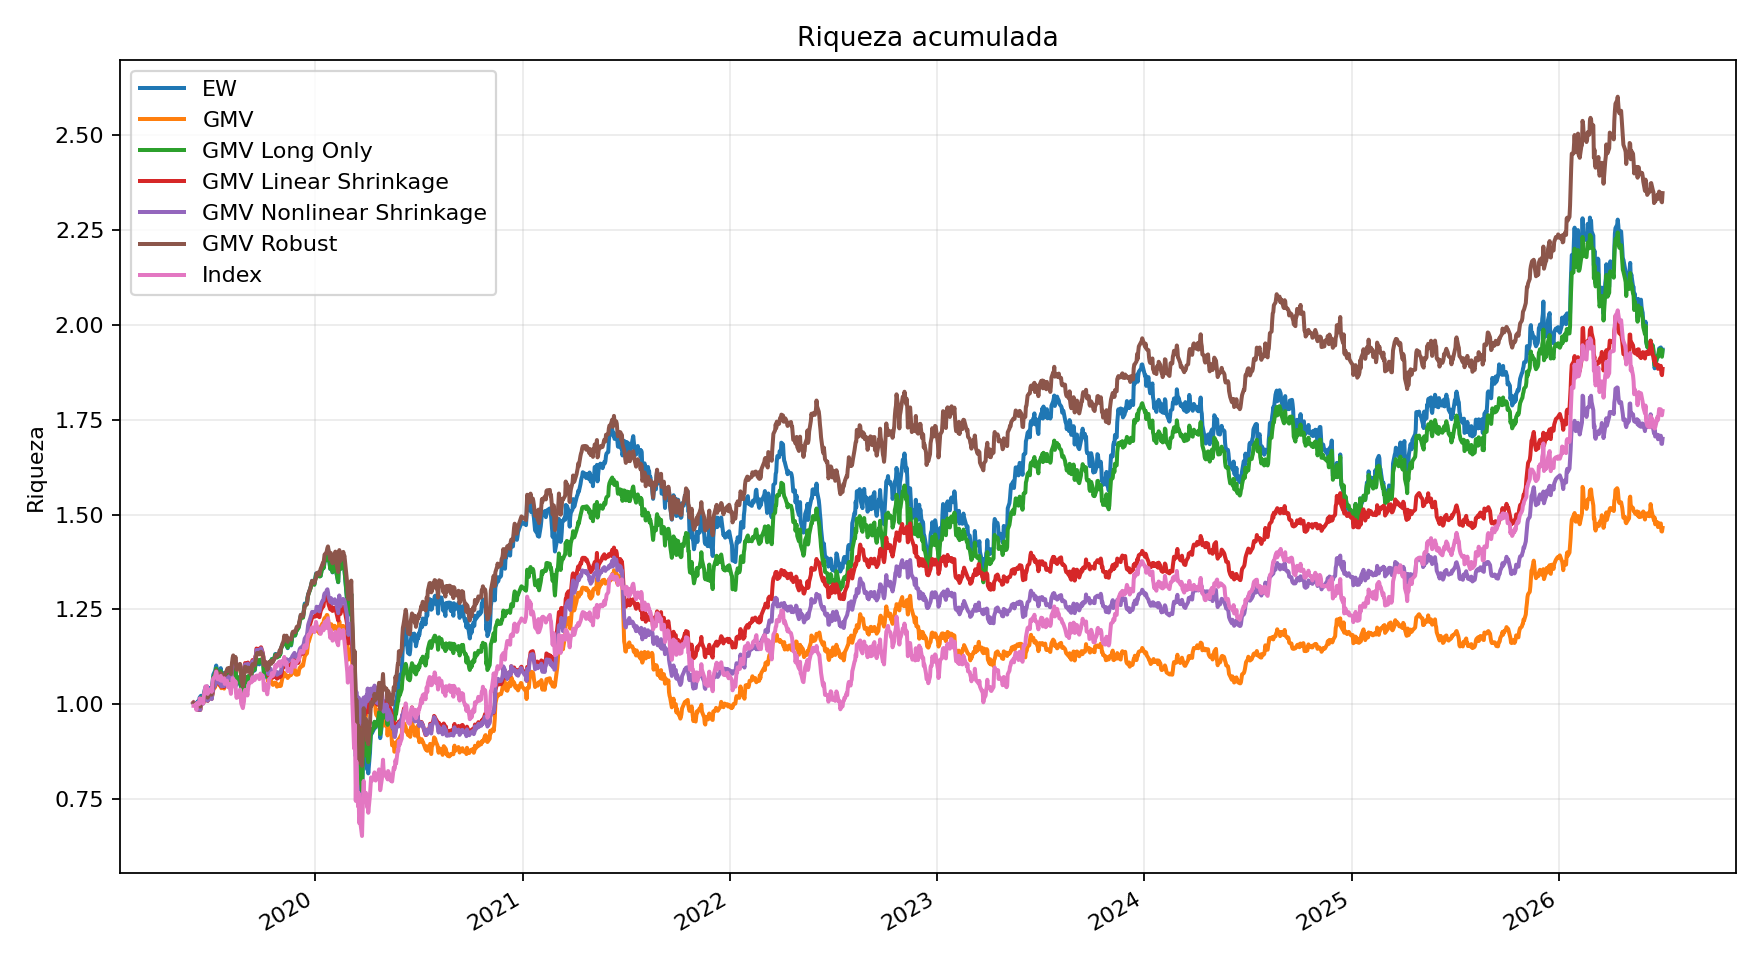
\includegraphics[width=0.92\textwidth]{outputs/figures/window_252/cumulative_wealth.png}
  \caption{Riqueza acumulada líquida para a janela de estimação $T=252$.}
  \label{fig:wealth252}
\end{figure}

A Figura~\ref{fig:turnover252} mostra o turnover ao longo do tempo. O ponto central do paper
é que uma carteira pode parecer boa antes de custos, mas tornar-se pouco atraente se exige
trocas excessivas de posição. Por isso, turnover não é uma métrica acessória: ele mede a
estabilidade operacional da regra de investimento.

\begin{figure}[htbp]
  \centering
  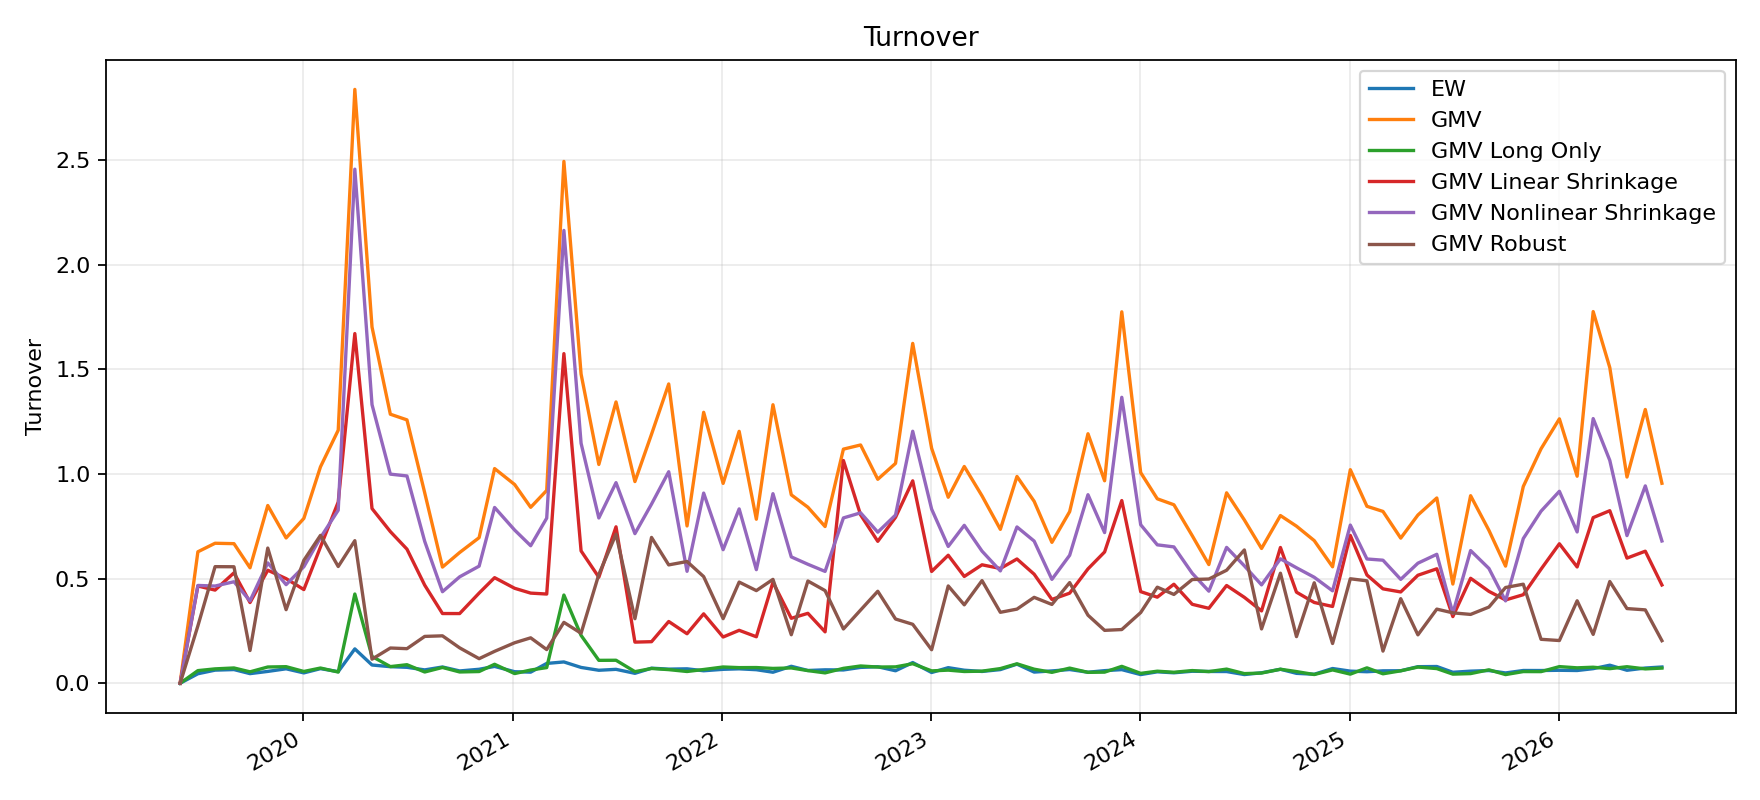
\includegraphics[width=0.92\textwidth]{outputs/figures/window_252/turnover.png}
  \caption{Turnover das carteiras para a janela $T=252$.}
  \label{fig:turnover252}
\end{figure}

A Figura~\ref{fig:weights252} resume o comportamento dos pesos da carteira robusta. Como o
método robusto não impõe a restrição long-only, pesos negativos podem aparecer. Isso não é
um erro: eles correspondem a posições vendidas, permitidas pelo problema GMV com apenas a
restrição orçamentária $\one^\top w=1$. A interpretação estatística é que o método tenta
reduzir a variância total da carteira usando a estrutura de covariância estimada de modo
robusto.

\begin{figure}[htbp]
  \centering
  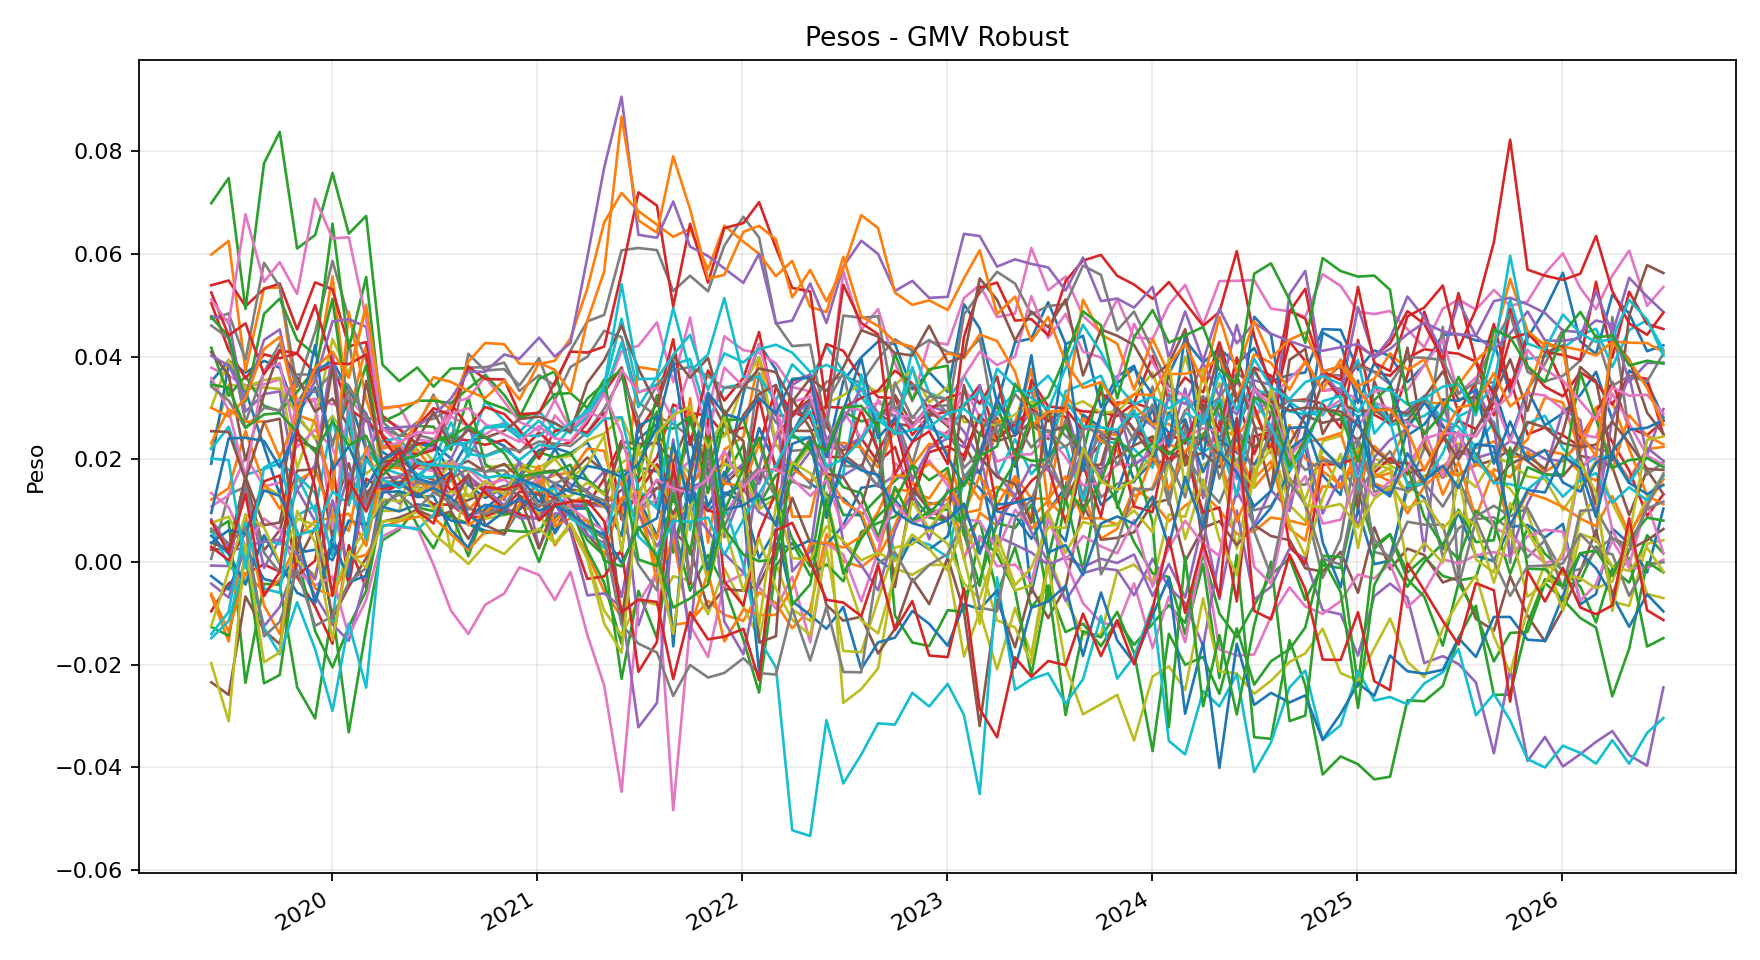
\includegraphics[width=0.92\textwidth]{outputs/figures/window_252/weights_gmv_robust.png}
  \caption{Pesos da carteira GMV Robust ao longo do tempo para $T=252$.}
  \label{fig:weights252}
\end{figure}

\begin{figure}[htbp]
  \centering
  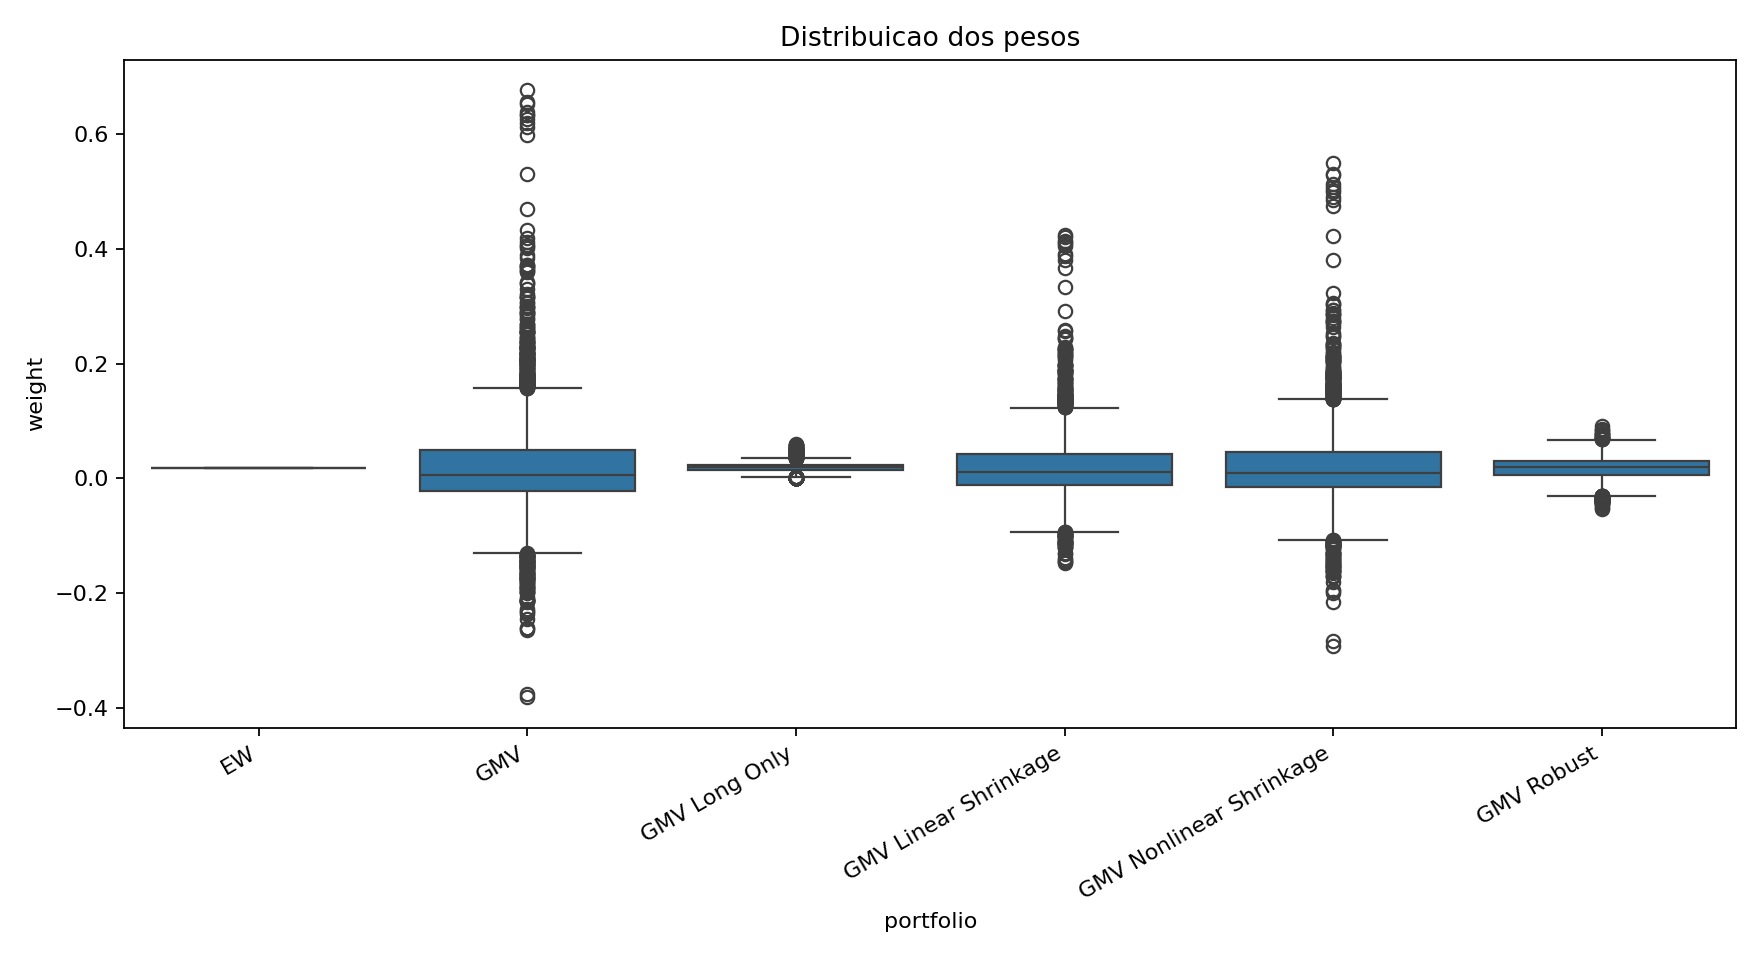
\includegraphics[width=0.82\textwidth]{outputs/figures/window_252/weight_distribution.png}
  \caption{Distribuição dos pesos das carteiras para $T=252$.}
  \label{fig:distweights252}
\end{figure}

\subsection{\texorpdfstring{Janela $T=500$}{Janela T=500}}

\begin{table}[htbp]
\centering
\caption{Resultados líquidos das carteiras para janela de estimação $T=500$.}
\label{tab:resultados-500}
\begin{tabular}{lrrrr}
\toprule
Carteira & Sharpe & Calmar & TO & TTO \\
\midrule
EW & 0.596 & 0.465 & 0.064 & 0.000 \\
GMV & 0.892 & 0.447 & 0.495 & 0.451 \\
GMV Long Only & 0.713 & 0.629 & 0.064 & 0.019 \\
GMV Linear Shrinkage & 1.010 & 0.570 & 0.335 & 0.292 \\
GMV Nonlinear Shrinkage & 0.956 & 0.501 & 0.425 & 0.383 \\
GMV Robust & 0.932 & 0.824 & 0.280 & 0.266 \\
Index & 0.708 & 0.453 & 0.000 & 0.000 \\
\bottomrule
\end{tabular}
\end{table}

Para $T=500$, a carteira robusta tem turnover menor que GMV e shrinkage e apresenta o maior
Calmar entre as carteiras reportadas. Esse padrão é alinhado com a motivação do artigo:
estabilizar pesos e reduzir custos, preservando desempenho fora da amostra.

\subsubsection{Gráficos para \texorpdfstring{$T=500$}{T=500}}

Com $T=500$, a janela de estimação é mais longa. Isso tende a reduzir ruído estatístico, pois
cada covariância é estimada com mais observações, mas também pode tornar a carteira mais lenta
para reagir a mudanças recentes de mercado. A Figura~\ref{fig:wealth500} mostra a riqueza
acumulada líquida nesse cenário.

\begin{figure}[htbp]
  \centering
  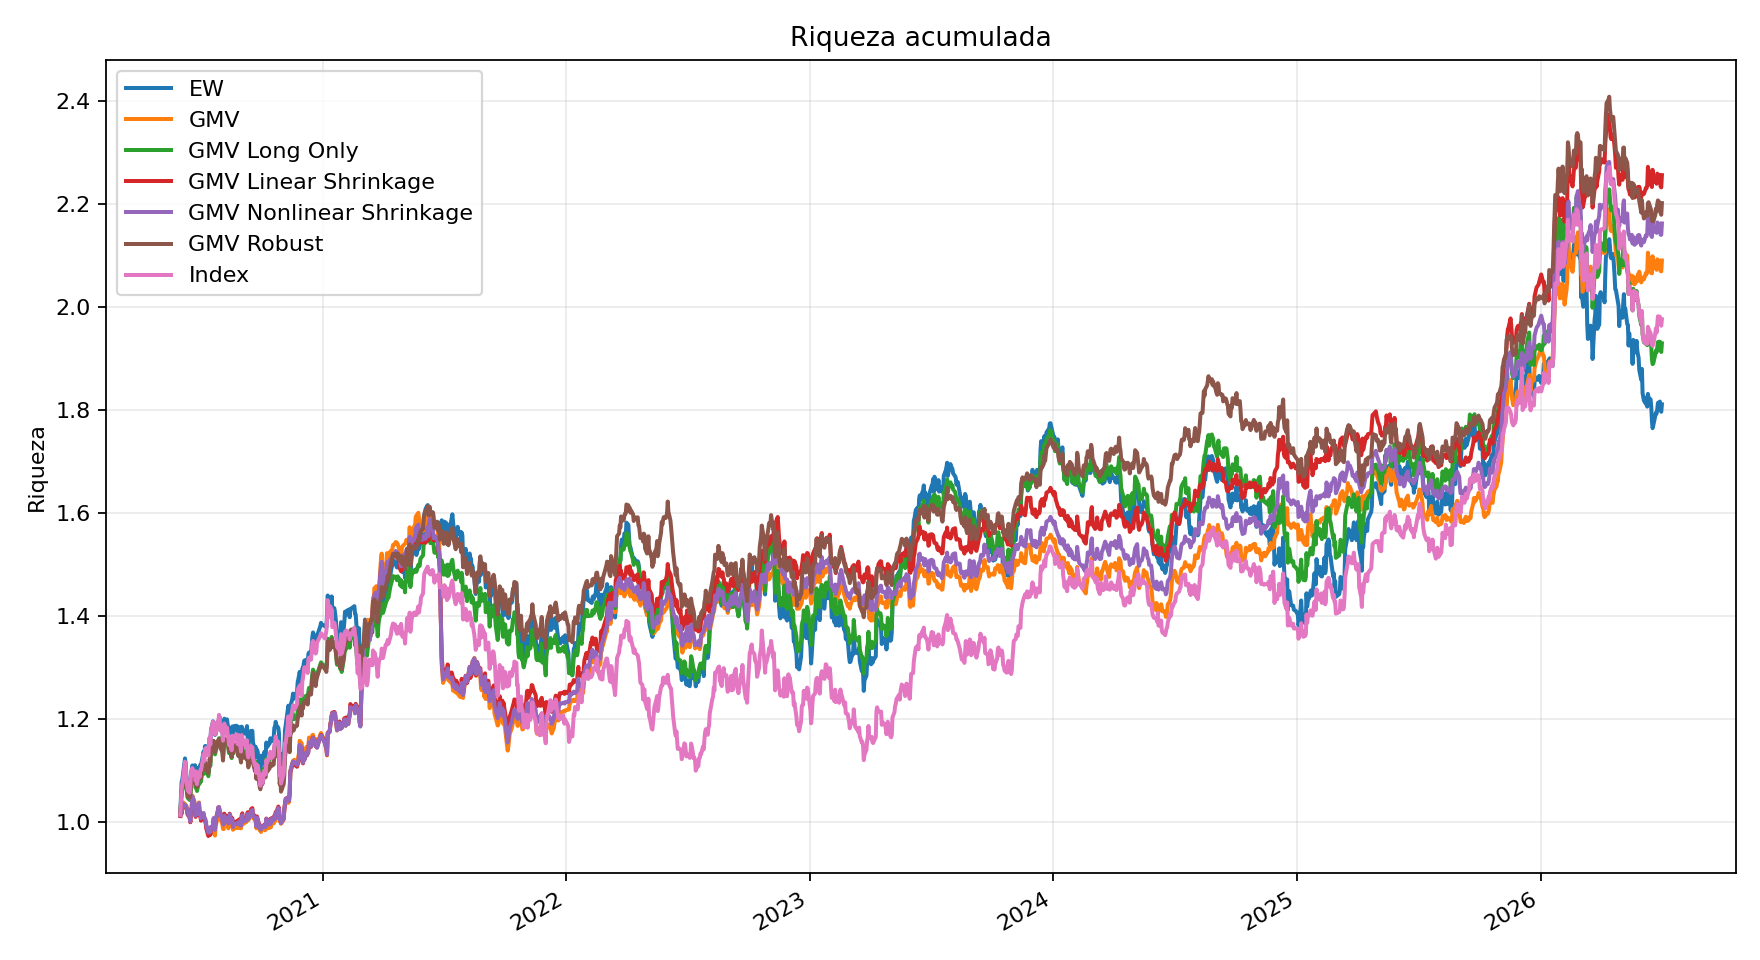
\includegraphics[width=0.92\textwidth]{outputs/figures/window_500/cumulative_wealth.png}
  \caption{Riqueza acumulada líquida para a janela de estimação $T=500$.}
  \label{fig:wealth500}
\end{figure}

A Figura~\ref{fig:turnover500} reforça uma das conclusões mais importantes do experimento:
com janela maior, a carteira robusta mantém turnover inferior ao dos métodos GMV amostral e
shrinkage, ao mesmo tempo em que preserva desempenho competitivo. Em termos práticos, isso
significa que a robustificação não está apenas melhorando uma métrica estatística abstrata;
ela está produzindo uma regra de alocação menos instável.

\begin{figure}[htbp]
  \centering
  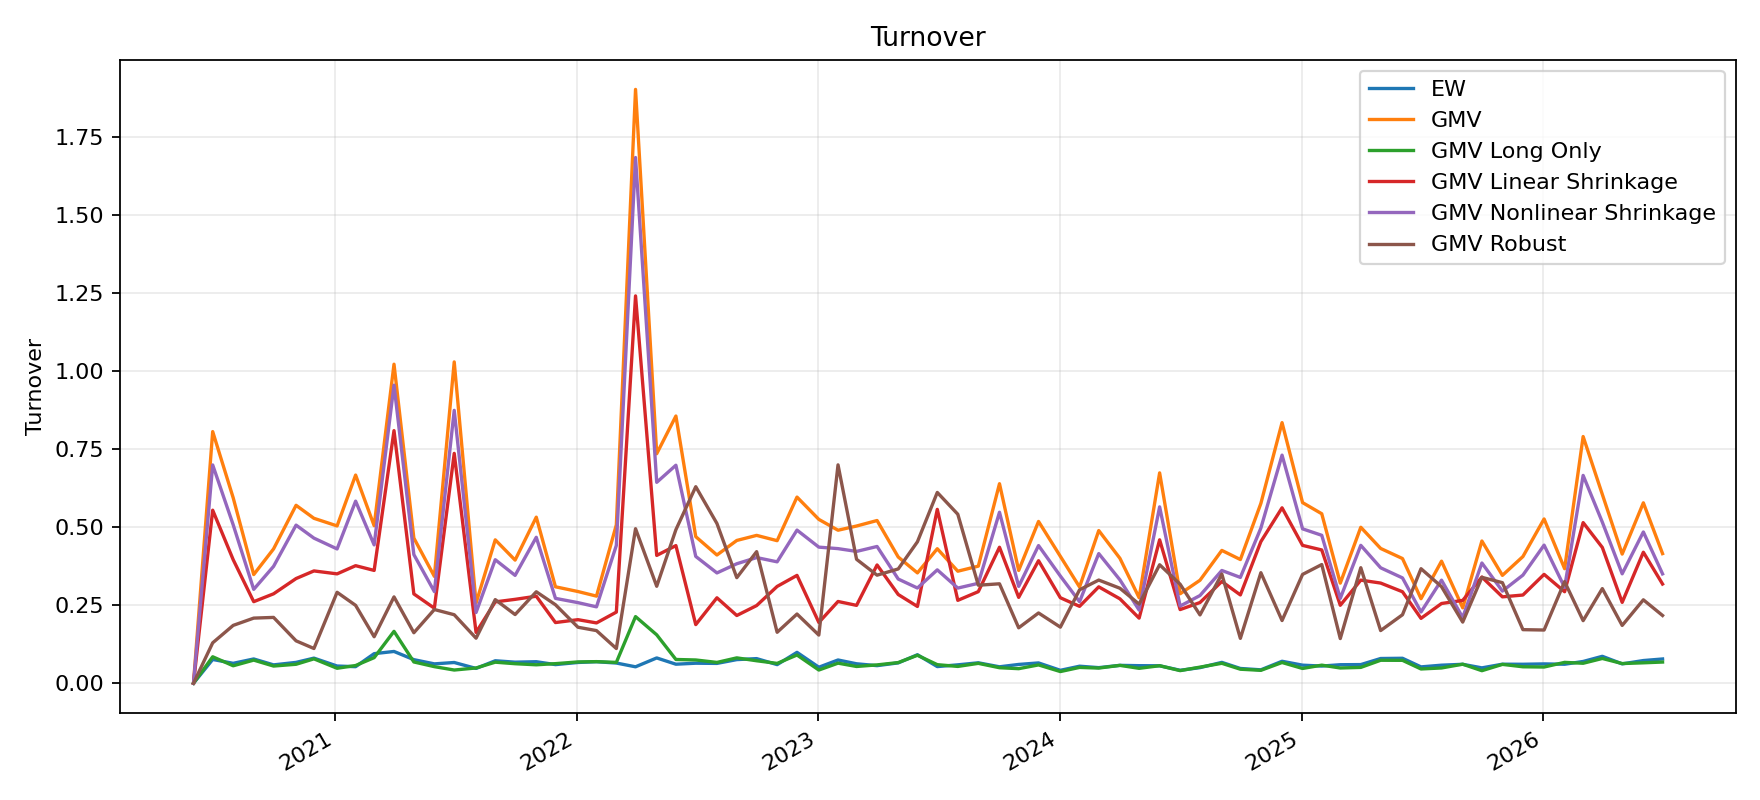
\includegraphics[width=0.92\textwidth]{outputs/figures/window_500/turnover.png}
  \caption{Turnover das carteiras para a janela $T=500$.}
  \label{fig:turnover500}
\end{figure}

\begin{figure}[htbp]
  \centering
  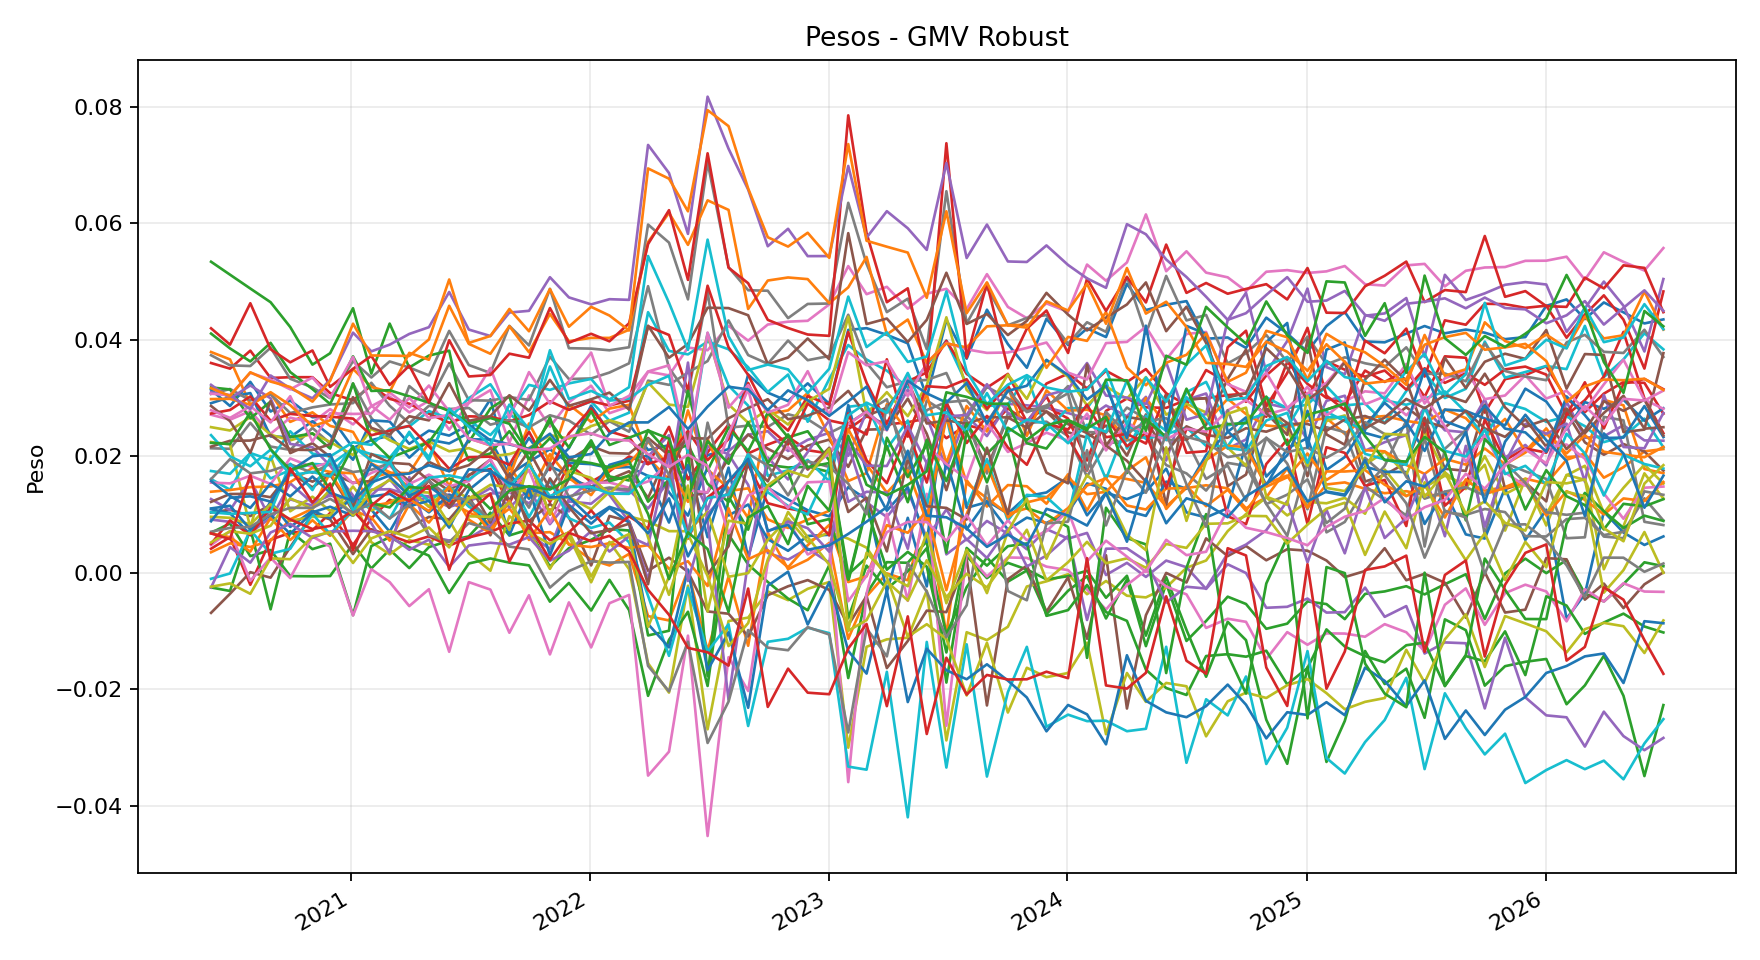
\includegraphics[width=0.92\textwidth]{outputs/figures/window_500/weights_gmv_robust.png}
  \caption{Pesos da carteira GMV Robust ao longo do tempo para $T=500$.}
  \label{fig:weights500}
\end{figure}

\begin{figure}[htbp]
  \centering
  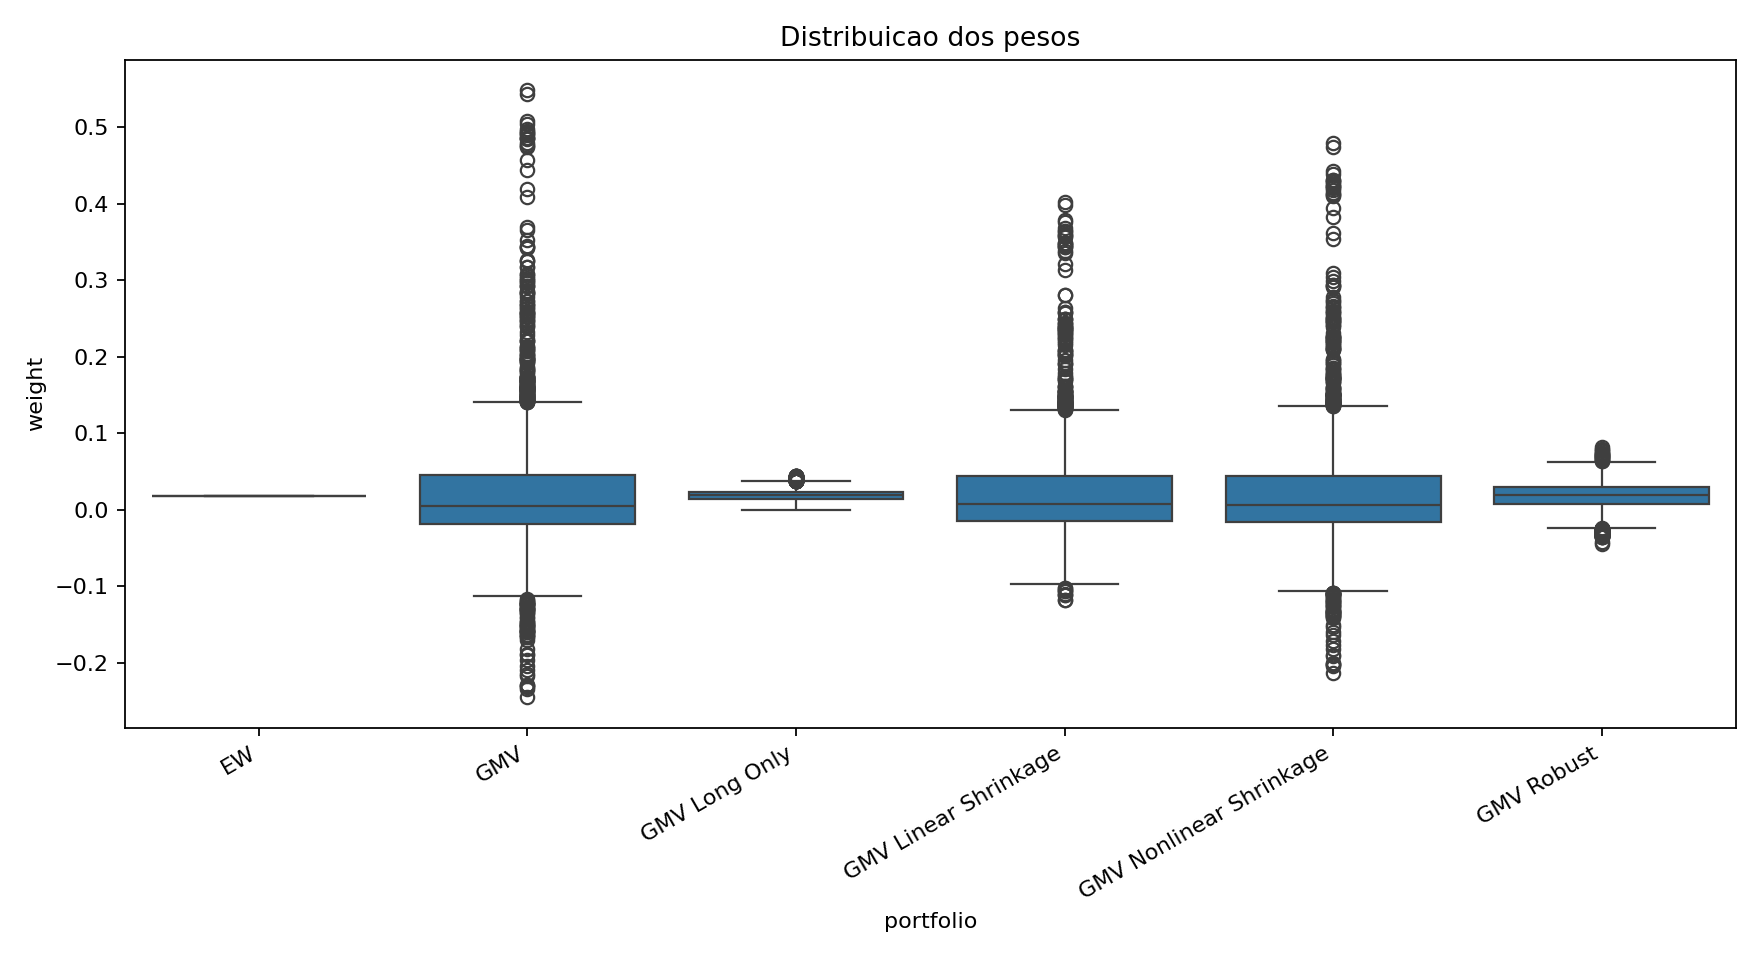
\includegraphics[width=0.82\textwidth]{outputs/figures/window_500/weight_distribution.png}
  \caption{Distribuição dos pesos das carteiras para $T=500$.}
  \label{fig:distweights500}
\end{figure}

\section{Conclusões do experimento}

O experimento confirma, nos dados brasileiros usados neste trabalho, a mensagem principal
do artigo \emph{Robustifying Markowitz}: em carteiras de mínima variância, a dificuldade
central não é apenas resolver o problema quadrático, mas estimar de modo estável o objeto que
entra no gradiente. O método robusto evita depender diretamente da inversão de uma matriz de
covariância ruidosa e, em vez disso, estima robustamente $\Sigma w$ a cada passo do PGD.

À luz da hipótese de pesquisa, a evidência empírica é favorável, mas não absoluta. A carteira
GMV Robust apresenta menor instabilidade que GMV amostral e que os métodos de shrinkage nas
duas janelas analisadas, quando a instabilidade é medida por turnover e target turnover. Em
desempenho líquido, a robusta domina os benchmarks em alguns critérios, como Sharpe em
$T=252$ e Calmar em $T=500$, mas não domina todos os critérios simultaneamente. Assim, a
conclusão adequada é que a hipótese é \textbf{parcialmente sustentada}: há evidência clara de
maior estabilidade e evidência competitiva de desempenho líquido fora da amostra, embora a
superioridade não seja uniforme em todas as métricas.

Para a janela $T=252$, a carteira GMV Robust obteve o maior Sharpe líquido entre as carteiras
reportadas. Ela também reduziu fortemente o turnover em relação à GMV amostral e às carteiras
de shrinkage. Esse resultado é pedagogicamente importante: robustez não significa apenas
``ignorar outliers''. Neste projeto, robustez significa construir uma regra de decisão menos
sensível a blocos de observações extremos ou instáveis.

Para a janela $T=500$, a carteira de shrinkage linear apresentou o maior Sharpe, mas a GMV
Robust apresentou o maior Calmar e menor turnover que GMV, shrinkage linear e nonlinear
shrinkage. Isso sugere uma conclusão mais fina: o método robusto não domina todos os critérios
em todos os cenários, mas entrega uma combinação atraente de desempenho, controle de drawdown
e estabilidade de pesos. Em aplicações reais, essa combinação pode ser mais relevante do que
maximizar apenas Sharpe.

O benchmark do índice também é importante. Comparar somente carteiras otimizadas entre si
pode esconder o fato de que uma regra sofisticada precisa superar uma alternativa simples e
investível. Nos dois tamanhos de janela, as carteiras otimizadas mais estáveis entregam
métricas competitivas contra o índice, mas com perfis diferentes de risco, turnover e
drawdown.

A principal conclusão técnica é que o projeto está coerente com a lógica matemática do paper:
usa PGD, projeção orçamentária, estimação robusta da ação $\Sigma w$, agregação HLZ/spectral
reweighting, rebalanceamento mensal, custos de transação e comparação com benchmarks
clássicos. O diferencial deste estudo é trocar o universo empírico original por ativos
brasileiros, preservando a estrutura conceitual do experimento.

\section{Validações metodológicas}

\subsection{Auditoria HLZ}

Para verificar o comportamento do agregador HLZ, foi construído um exemplo contaminado e
avaliado se o procedimento:

\begin{itemize}[leftmargin=*]
  \item respeita o cap de pesos em $W_{\ell,\epsilon}$;
  \item reduz a norma espectral ponderada em relação aos pesos uniformes.
\end{itemize}

Na última execução, o raio ponderado uniforme foi $27.151586$ e o raio ponderado HLZ foi
$1.615178$, com peso máximo $0.149461$ e cap $0.150000$.

\subsection{Validação do nonlinear shrinkage}

O estimador de nonlinear shrinkage foi validado verificando duas propriedades fundamentais da
matriz estimada: simetria e autovalores positivos. Essas condições são importantes porque uma
matriz de covariância deve ser simétrica e semidefinida positiva. Também foi prevista a
possibilidade de comparação contra uma matriz de referência externa, caso uma implementação
oficial do estimador seja usada como base de validação.

\section{Limitações e pontos de atenção}

O projeto está alinhado com a lógica central do artigo, mas há pontos que devem ser lidos
com cuidado:

\begin{enumerate}[leftmargin=*]
  \item O nonlinear shrinkage usa uma implementação espectral interna. Para validação numérica
  literal, deve-se comparar contra a implementação original de Ledoit--Wolf.
  \item A truncagem robusta usa quantil empírico da norma, pois o parâmetro teórico exato depende
  de constantes desconhecidas na prática.
  \item O universo brasileiro é congelado com ativos que passaram pelo filtro de histórico. Essa é
  uma escolha de reprodutibilidade, mas não é uma carteira teórica dinâmica da B3.
  \item A fonte de preços pode revisar ou ajustar séries históricas; por isso a preservação das
  bases usadas no estudo é parte importante da reprodutibilidade.
  \item O custo computacional do HLZ é maior que o de uma mediana coordenada simples. Isso é
  esperado, pois o método usa autovalores/autovetores e reponderação iterativa.
\end{enumerate}

\section{Conclusão}

Este trabalho implementa uma versão aplicada ao Brasil da lógica de \emph{Robustifying
Markowitz}. A contribuição central é substituir a dependência direta em $\Sigmahat^{-1}$ por
um procedimento iterativo que estima robustamente $\Sigma w$. Essa troca é fundamental em
ambientes com alta dimensão, amostras finitas e caudas pesadas.

Para alunos iniciando em Estatística Robusta, o projeto ilustra três ideias importantes:

\begin{enumerate}[leftmargin=*]
  \item robustez não é apenas ``remover outliers'', mas controlar a influência deles em um problema
  de otimização;
  \item em alta dimensão, estimar uma matriz inteira pode ser mais difícil do que estimar sua ação
  em direções relevantes;
  \item métricas financeiras como turnover e custos de transação são parte essencial da avaliação
  estatística de carteiras.
\end{enumerate}

O resultado final é um procedimento reprodutível que combina teoria robusta moderna, otimização
convexa e avaliação empírica em dados brasileiros.

\begin{thebibliography}{9}

\bibitem{markowitz1952}
Markowitz, H. (1952).
\newblock Portfolio Selection.
\newblock \emph{The Journal of Finance}, 7(1), 77--91.

\bibitem{ledoitwolf2004}
Ledoit, O. and Wolf, M. (2004).
\newblock A well-conditioned estimator for large-dimensional covariance matrices.
\newblock \emph{Journal of Multivariate Analysis}, 88(2), 365--411.

\bibitem{ledoitwolf2017}
Ledoit, O. and Wolf, M. (2017).
\newblock Nonlinear shrinkage of the covariance matrix for portfolio selection: Markowitz meets Goldilocks.
\newblock \emph{The Review of Financial Studies}, 30(12), 4349--4388.

\bibitem{ledoitwolf2008}
Ledoit, O. and Wolf, M. (2008).
\newblock Robust performance hypothesis testing with the Sharpe ratio.
\newblock \emph{Journal of Empirical Finance}, 15(5), 850--859.

\bibitem{ledoitwolf2011}
Ledoit, O. and Wolf, M. (2011).
\newblock Robust performance hypothesis testing with the variance.
\newblock \emph{Wilmott}, 2011(55), 86--89.

\bibitem{hlz2020}
Hopkins, S. B., Li, J. and Zhang, F. (2020).
\newblock Robust and Heavy-Tailed Mean Estimation Made Simple, via Regret Minimization.
\newblock arXiv:2007.15839.

\bibitem{robustifyingmarkowitz}
Haerdle, W. K., Klochkov, Y., Petukhina, A. and Zhivotovskiy, N. (2022).
\newblock Robustifying Markowitz.
\newblock arXiv:2212.13996.

\bibitem{neweywest1987}
Newey, W. K. and West, K. D. (1987).
\newblock A simple, positive semi-definite, heteroskedasticity and autocorrelation consistent covariance matrix.
\newblock \emph{Econometrica}, 55(3), 703--708.

\end{thebibliography}

\end{document}
